%
% jacobi.tex
%
% (c) 2022 Prof Dr Andreas Müller, OST Ostsdchweizer Fachhochschule
%
\section{Jacobi-Polynome
\label{buch:integrale:subsection:jacobi-polynome}}
\rhead{Jacobi-Polynome}
Das $L^2$-Skalarprodukt von
Definition~\label{buch:orthogonal:def:skalarprodukt}
ist nicht das einzige Skalarprodukt von Funktionen, bezüglich dem 
orthogonale Funktionenfamilien konstruiert werden können.
Die Definition~\label{buch:orthogonal:def:skalarproduktw}
erlaubt, das Skalarprodukt mit einer Gewichtsfunktion
zu erweitern.

Auch in diesem Abschnitt geht es um Polynome, deren Werte auf
dem Intervall $(-1,1)$ interessieren.
Die Legendre-Polynome waren aus den Monomen konstruiert worden durch
Orthogonalisierung bezüglich des gewöhnlichen $L^2$-Skalarproduktes.
Die Normierung war einigermassen willkürlich gewählt worden und
hatte nichts mit dem Skalarprodukt zu tun.

\begin{figure}
\centering
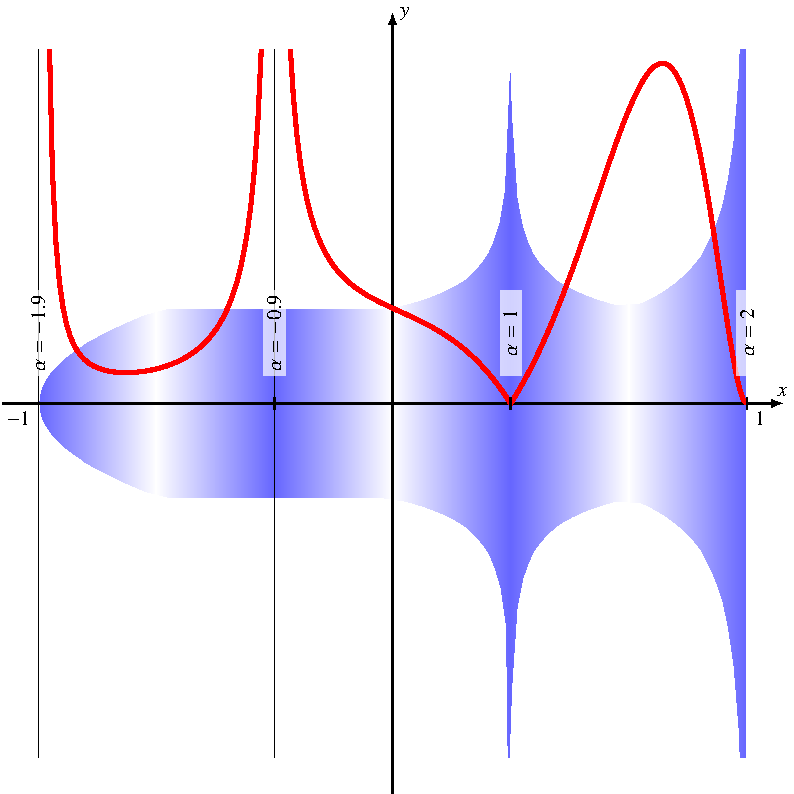
\includegraphics{chapters/070-orthogonalitaet/images/weight.pdf}
\caption{Nullstellen und Pole der Gewichtsfunktion (rot) legen Ort
und Grad von Polen und Nullstellen der Funktionen fest, die beschränkte
$\|\,\cdot\,\|_w$-Norm haben.
An den Stellen $\pm 1$ und $\pm\frac12$ hat die Gewichtsfunktion
Pole bzw.~Nullstellen mit Grad $\alpha$.
Der blaue Bereich deutet an, wie schnell die Funktion $f$ in diesem
Bereich anwachsen kann, bzw.~wie schnell nahe der Polstelle gegen $0$
gehen muss.
\label{buch:orthogonalitaet:fig:gewicht}}
\end{figure}
%
% Pole und Nullstellen der Gewichtsfunktion
%
\subsection{Pole und Nullstellen
\label{buch:orthogonal:pole-und-nullstellen}}
Das Skalarprodukt $\langle\,\;,\;\rangle_w$ ist nur sinnvoll
für Funktionen $f(x)$, für die die Norm $\|f\|_w$ definiert ist.
An einer Nullstelle $x_0$ der Gewichtsfunktion $w$ darf die Funktion $f$ 
einen Pol haben. 
Solange $f(x)$ für $x\to x_0$ nicht zu schnell divergiert, kann
das Produkt $|f(x)|^2 w(x)$ immer noch integrierbar sein.


Um dies etwas genauer zu quantifizieren, nehmen wir an, dass
$w(x)$ an der Stelle $x_0$ eine Nullstelle vom Grad $\alpha$ hat.
Dies bedeutet, dass $w(x) \approx C|x-x_0|^\alpha$ ist für eine geeignete
Konstante $C$ und für $|x-x_0|<\varepsilon$.
Ein Pol von $f$ vom Grad $a$ an der Stelle $x_0$ führt entsprechend auf
eine Abschätzung $|f(x)| \approx D|f(x)|^{-a}$ für $|x-x_0|<\varepsilon$.
Dann ist
\[
|f(x)|^2 w(x) \approx CD |x-x_0|^{\alpha-2a}.
\]
Für das Integral in der Nähe von $x_0$ ist
\begin{align*}
\int_{x_0-\varepsilon}^{x_0+\varepsilon}
|f(x)|^2 w(x)\,dx
&\approx 
CD
\int_{x_0-\varepsilon}^{x_0+\varepsilon}
|x-x_0|^{\alpha-2a}\,dx
\\
&=
2CD
\int_0^\varepsilon
t^{\alpha-2a}
\,dt
=
2CD
\begin{cases}
\displaystyle
\;
\biggl[\frac{t^{\alpha-2a+1}}{\alpha-2a+1}\biggr]_0^\varepsilon
&\qquad
\alpha-2a\ne-1
\\[7pt]
\displaystyle
\;
\biggl[ \log t \biggr]_0^\varepsilon
&\qquad
\text{sonst.}
\end{cases}
\end{align*}
Der Zähler $t^{\alpha-2a+1}$ divergiert für $t\to 0$ genau dann,
wenn $\alpha-2a+1<0$ oder $\alpha<2a-1$.
Auch im zweiten Fall, für $\alpha-2a+1=0$, divergiert das Integral.
Damit die Norm $\|f\|_w$ definiert ist, muss also $a<\frac12(\alpha+1)$
sein.

Ganz ähnlich führt eine Polstelle von $w$ vom Grad $\alpha$
an der Stelle $x_0$ dazu, dass $f$ dort eine Nullstelle vom Grad
$a$ haben muss.
Das Normintegral konvergiert nur, wenn $2a-\alpha > -1$ ist
oder $a > \frac12(\alpha+1)$.
 
Pole der Gewichtsfunktion schränken also ein, welche Funktionen
überhaupt der Untersuchung mit Hilfe des Skalarproduktes
$\langle\,\;,\;\rangle_w$ zugänglich sind
(Abbildung~\ref{buch:orthogonalitaet:fig:gewicht}).
Ist die Ordnung $\alpha$ des Poles grösser als $1$, dann müssen die Funktionen
eine Nullstelle mindestens vom Grad $\frac12(a+1)$ haben.
Nullstellen der Gewichtsfunktion erweitern die Klasse der Funktionen.
Ist die Ordnung der Nullstelle $\alpha$, dann dürfen die Funktionen einen
Pol der Ordnung kleiner als $\frac12(\alpha+1)$ haben.


%
% Die Jacobische Gewichtsfunktion
%
\subsection{Jacobische Gewichtsfunktion}
Die Gewichtsfunktion für die Legendrepolynome war $w(x)=1$, alle
Punkte im Intervall $(-1,1)$ hatten das gleiche Gewicht.
Diese soll jetzt ersetzt werden durch eine Gewichtsfunktion, die
den Punkten an den Intervallenden mehr oder weniger Gewicht gibt,
wobei auch zugelassen sein soll, dass die Gewichtung nicht symmetrisch
ist.

\begin{definition}
Die {\em Jacobi-Gewichtsfunktion} ist die Funktion
\[
w^{(\alpha,\beta)}
\colon (-1,1)\to\mathbb{R}
:
x\mapsto w^{(\alpha,\beta)}(x) = (1-x)^\alpha(1+x)^\beta
\]
mit $\alpha,\beta\in\mathbb{R}$.
Das Skalarprodukt zugehörige Skalarprodukt wird auch als
\[
\langle\,\;,\;\rangle_{w^{(\alpha,\beta)}}
=
\langle\,\;,\;\rangle_{(\alpha,\beta)}
\]
bezeichnet und die zugehörige Norm mit
\[
\|f\|_{(\alpha,\beta)}
=
\langle f,f\rangle_{(\alpha,\beta)}
=
\int_{-1}^1 |f(x)|^2 w^{(\alpha,\beta)}(x)\,dx.
\]
\end{definition}

\begin{definition}
Die {\em Jacobi-Polynome} $P^{(\alpha,\beta)}_n(x)$ sind 
Polynome vom Grad $n$, die bezüglich des Skalarproduktes
$\langle\,\;,\;\rangle_{w^{(\alpha,\beta)}}$ orthogonal sind
und mit
\[
P_n^{(\alpha,\beta)}(1) = \binom{n+\alpha}n
\]
normiert sind.
\end{definition}

Für $\alpha=\beta=0$ entsteht die Gewichtsfunktion
$w^{(0,0)}(x)=1$, die Legendre-Polynome sind also der Spezialfall
$\alpha=\beta=0$ der Jacobi-Polynome.

Der Exponent $\alpha$ in der Gewichtsfunktion $w^{(\alpha,\beta)}(x)$
steuert das Gewicht, welches Punkte am rechten Rand des Intervalls
erhalten.
Für positive Werte von $\alpha$ hat $w^{(\alpha,\beta)}(x)$ eine
Nullstelle vom Grad $\alpha$ an der Stelle $x=1$, nach
Abschnitt~\ref{buch:orthogonal:pole-und-nullstellen}
dürfen die Funktionen einen Pole der Ordnung $<\frac12(\alpha-1)$ haben.
Je grösser $\alpha$ ist, desto weniger Gewicht haben die Punkte
am rechten Rand des Intervalls und desto schneller darf eine Funktion
für $x\to 1$ divergieren.

Für negative Werte von $\alpha$ hat $w^{(\alpha,\beta)}(x)$ einen
Pol vom Grad $-\alpha$ an der Stelle $x=1$.
Funktionen müssen daher also ein Nullstelle mindestens vom Grad
$\frac12(1-\alpha)$ haben.

\begin{figure}
\centering
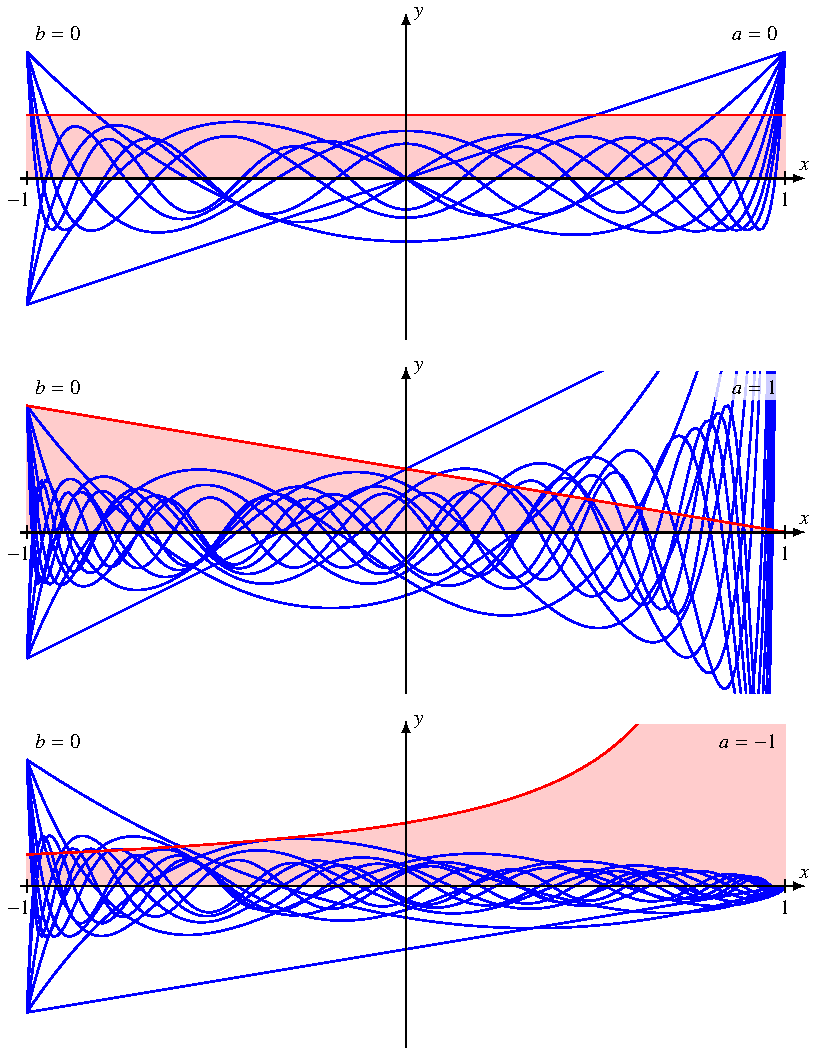
\includegraphics[width=\textwidth]{chapters/070-orthogonalitaet/images/jacobi.pdf}
\caption{Jacobi-Polynome vom Grad $1$ bis $14$ für verschiedene Werte
der Parameter $\alpha$ und $\beta$.
Je grösser $\alpha$, desto weniger Gewicht bekommen die Funktionswerte am
rechten Rand und desto grösser werden die Funktionswerte.
Für negative $\alpha$ müssen die Polynome dagegen eine Nullstelle am
rechten Rand haben.
\label{buch:orthogonal:fig:jacobi-parameter}}
\end{figure}

\subsection{Jacobi-Gewichtsfunktion und Beta-Verteilung
\label{buch:orthogonal:subsection:beta-verteilung}}
Die Jacobi-Gewichtsfunktion entsteht aus der Wahrscheinlichkeitsdichte
der Beta-Verteilung, die in
Abschnitt~\ref{buch:rekursion:subsection:beta-verteilung}
eingeführt wurde mit Hilfe der Variablen-Transformation $x = 2t-1$
oder $t=(x+1)/2$.
Das Integral mit der Jacobi-Gewichtsfunktion $w^{(\alpha,\beta)}(x)$ 
kann damit umgeformt werden in
\[
\int_{-1}^1
f(x)\,w^{(\alpha,\beta)}(x)\,dx
=
\int_0^1
f(2t-1) w^{(\alpha,\beta)}(2t-1)\,2\,dt
=
\int_0^1
f(2t-1)
(1-(2t-1))^\alpha (1+(2t-1))^\beta
\,2\,dt
\]

%
% 
%
\subsection{Jacobi-Polynome niedrigen Grades}
In Abbildung~\ref{buch:orthogonal:fig:jacobi-parameter}
ist die Abhängigkeit der Jacobi-Polynome von den Parametern $a$ und $b$
illustriert.

%
%
%
\subsection{Rekursionsformel}
\url{https://ch.mathworks.com/help/symbolic/sym.jacobip.html;jsessionid=9ef5241a38b49d65f6f61cba98c8}

%
%
%
\subsection{Jacobi-Polynome als hypergeometrische Funktionen}

%
%
%
\subsection{Jacobi-Differentialgleichung}

%
%
%
\subsection{Ableitung und Rodrigues-Formel}




